\documentclass[12pt,a4paper,twoside]{article}

\usepackage[applemac]{inputenc}
\usepackage[T1]{fontenc}
\usepackage[english]{babel}

\usepackage{enumerate}
\usepackage{amsthm}  
\usepackage{amssymb}  
\usepackage{amsmath}
\usepackage{graphicx}
\usepackage{biblatex}


\theoremstyle{plain}
\newtheorem{thm}{Theorem}



\theoremstyle{definition}
\newtheorem{defin}{Definition}
\newtheorem*{defin*}{Definition}

\theoremstyle{remark}
\newtheorem{oss}{Remark}


\linespread{1.3}                       
\oddsidemargin=30pt \evensidemargin=30pt 
\hyphenation{}                          

\begin{document}


\section*{Replicator dynamics and Evolutionary Stable States}
Let us consider an infinite population with $N$ types of individuals, where the fitness of an individual of type $i$ when interacting with an individual of type $j$ is given by $A_{ij}$.
The replicator dynamics equation is given by:
\begin{align}
\dot {x_i}=x_{i}[f_i(x)-\phi (x)], \label{repl_eq}\tag{RE}
\end{align}
with $\phi (x)=\sum _{j=1}^{n}{x_j f_j(x)}$ being the average fitness in population and $f_i(x)$
being the population dependent fitness of individuals of type $i$
\begin{align*}
f_i(x) := (Ax)_i
\end{align*}
The unit symplex $\Delta$ is invariant under the flow of replicator dynamics (see \cite{HS98}, section 7.1); in what follows we will consider its restriction to points in $m$-dimensional symplex $\Delta^m \subset \mathbb{R}^{m+1}$.


\begin{defin*}A point $x \in \Delta^m$ is called \textit{Nash equilibrium} if
\begin{align*}
\langle x, A \hat{x} \rangle \geq \langle \hat{x}, A\hat{x} \rangle
\end{align*}
and \textit{evolutionary stable state} (ESS) if
\begin{align*}
\langle x, A \hat{x} \rangle > \langle \hat{x}, A\hat{x} \rangle
\end{align*}
for all $\hat{x}$ in a neighbourhood of $x$. 
\end{defin*}
Clearly ESS is a stronger condition than Nash equilibrium. A population state is evolutionary stable  %(also known as convergence stability) 
when all of the strategies used within the population have equal fitness and the equilibrium is stable under small perturbations. This concept has key importance in fields like behavioural ecology, evolutionary psychology, mathematical game theory and economics.
ESSs are tightly related to replicator dynamics, indeed  
\begin{thm}[\cite{HS98}, section 7.2] If $x \in \Delta^m$ is a Nash equilibrium, then it is a rest point of (\ref{repl_eq}) 
\end{thm}


\section*{Neural Networks for rest point detections}
Neural Networks provide a convenient way to detect critical points of a real valued function via gradient descent. Let us use them to detect critical points of (\ref{repl_eq}) by first define the NN architecture and loss function.

\begin{paragraph}{NN Architecture}
\begin{enumerate}[i)]
\item  $m+1$ neurons $x_i$ in input layer, each of them representing the relative frequency of strategy $i$ in the population
\item a sequence of hidden fully connected layers
\item  $m+1$ neurons $y_i$ in output layer, each of them representing the relative frequency of strategy $i$ in the population.
\end{enumerate}

\begin{figure}[h]
\centering
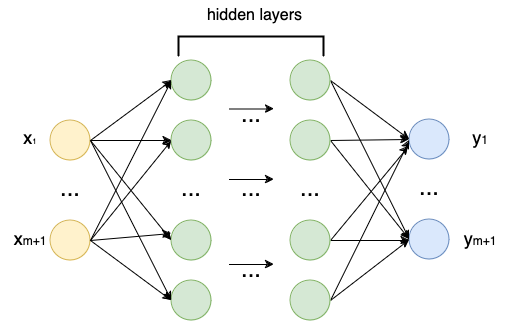
\includegraphics[scale=0.6]{figures/feedforward_nn_architecture.png}
\caption{NN architecture}
\label{nn_arch}
\end{figure} 
\end{paragraph}

\begin{paragraph}{Loss} \ \\
Let $x =(x_1, \ldots, x_{m+1}) \in \Delta^m$, we define a function $l: \mathbb{R}^{m+1} \rightarrow \mathbb{R}$ as 
\begin{align}
l(x) := \sum_{i=1}^{m+1} \sum_{j=1}^{m+1} (f_i(x) -f_j(x))^2 sign(x_i) sign(x_j)  
\end{align}
and notice its zeros correspond to rest points of (\ref{repl_eq}), indeed $x$ is a rest point of replicator equations iff
\begin{align*}
x_i = 0 \textrm{ or } f_{i}(x)-\phi (x) = 0
\end{align*}
for each $i = 1,\ldots, m+1$.\\
The function $l$ is non negative when restricted to $\Delta^m$, hence its zeros coincide with minima (thus critical points).
\end{paragraph}
At fit stage the output layer is iteratively updated to minimize the loss and we call $p$ its representation at last training epoch. If loss vanishes on $p$, then $p$ is a critical point of (\ref{repl_eq}) and then a potential ESS, since 
\begin{align*}
\textrm{ESS}  \subseteq \textrm{Nash equilibrium} \subseteq  \textrm{rest point of (\ref{repl_eq}) } 
\end{align*}

\section*{ESS condition on rest points}
Assuming a rest point $x \in \Delta^n$ is detected at optimization step, we wish to see if it is an ESS, by checking that $x$ is a local minimum for the function $g_x:\Delta^m \rightarrow \mathbb{R}$ defined as
\begin{align*}
g_x(y) :=  \langle x, A y \rangle  - \langle y, A y \rangle
\end{align*} 
This is done by
\begin{enumerate}[1)]
\item  parametrizing a neighbourhood of $x$ using a linear function $L:\mathbb{R}^m \rightarrow \mathbb{R}^{m+1}$ such that $L(0) = x$, \label{cond_zero_grad}
\item checking that 0 is a critical point of $g_x \circ L$, whose Hessian is positive definite \label{cond_pos_hess}
\end{enumerate}
Assuming $x\in int(\Delta^n)$ is a rest point for (\ref{repl_eq}), the two conditions above are satisfied iff $x$ is ESS.


\section*{Extension to Graphs}
Let us consider a graph $G$ with:  
\begin{enumerate}[-]
\item  $n \geq 1$ nodes, each of them representing an infinite population, 
\item $\dfrac{n(n-1)}{2}$ oriented weighted edges representing connections (likelihood of interaction) between populations,  
\item $m\geq 1$ strategies being the allowed behaviours of individuals in population,  
\item $n$ payoff matrices (one for each node) prescribing the variation of fitness when two individuals meet.  
\end{enumerate}
Such a graph describes the fitness of different strategies in populations that are spatially linked and in which environment determines the payoff of a strategy.\\
If $n=1$ the graph consists of a single population, which is the original setting considered by Maynard Smith in his seminal work on ESS, see \cite{MS82}.\\
Given a node $i$, the $a^i_{j,k}$ entry of $n \times n$ adjacency matrix $A^i$ is the probability that an individual of node $j$ has of interacting with an individual of node $k$ (under rules of environment $k$).\\ 
ESS concept can be extended verbatim to graph setting. Just notice that in this setting plain feedforwards NN are not suitable for critical point detection, but Graph Neural Networks (https://distill.pub/2021/gnn-intro) provide a natural way to tackle the problem.
\begin{thebibliography}{999}


\bibitem{HS98}[HS98]
  J. Hofbauer, K. Sigmund,
  \emph{Evolutionary Games and Population Dynamics}.
  https://api.semanticscholar.org/CorpusID:85023742,
  1998.

\bibitem{TJ78}[TJ78]
  Taylor, P. D, Jonker, L. B.,
  \emph{Evolutionarily stable states and Game Dynamics}.
  Mathematical Biosciences 40, 145-156. https://doi.org/10.1016/0025-5564(78)90077-9,
  1978.


\bibitem{MS82}[MS82]
  J. Maynard Smith,
  \emph{Evolution and the Theory of Games}.
  https://api.semanticscholar.org/CorpusID:146179511,
  1982.  
  
  
  
% http://www.evolutionary-ecology.com/issues/v11/n04/ccar2445.pdf three main concepts ESS and stability
% reference https://nashpy.readthedocs.io/en/stable/text-book/replicator-dynamics.html

\end{thebibliography}

\end{document}


